\begin{mdframed}[style=warning]
	\begin{ejercicio}
		\textbf{Conceptos.}
		\begin{enumerate}
			\item La suma de las cargas en ambas placas de un capacitor es cero. ¿Qué almacena el capacitor? \\
			\textbf{R$//$} Almacena energía potencial eléctrica en forma de campo eléctrico.
			\item Ya que las cargas en las placas de un capacitor de placas paralelas tienen signo opuesto, se atraen. Por eso, debería efectuarse un trabajo positivo para incrementar la separación entre las mismas. ¿Qué tipo de energía se modifica en el sistema debido al trabajo externo efectuado en este proceso?
		\end{enumerate}
	\end{ejercicio}
\end{mdframed}






\begin{mdframed}[style=warning]
	\begin{ejercicio}
		\begin{multicols}{2}
			Un capacitor de aire variable utilizado en un circuito sintonizador de radio está hecho de $N$ placas semicirculares, cada una de radio $R$ y colocadas entre sí a una distancia $d$, y conectadas eléctricamente. Como puede observar en la figura, un segundo conjunto de placas idéntcas, está intercalado con el primer conjunto. Cada placa en el segundo juego está a la mitad de las del primer conjunto. El segundo conjunto puede girar como una sola unidad. Determine la capacidad como una función del ángulo de rotación $\theta$, en donde $\theta = 0$ corresponde a la posición de máxima capacitancia.
			\columnbreak
			\begin{figure}[H]
				\centering
				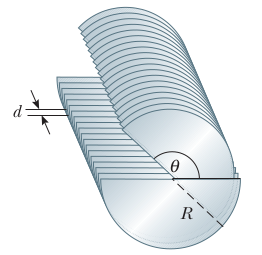
\includegraphics[scale=0.55]{./img/cap.png}
				\caption{Ejercicio 2, placas semicirculares.}
				\label{ej2}
			\end{figure}
		\end{multicols}
	\end{ejercicio}
	\textbf{Solución 2: } \\
	Para $\theta = 0$ se tiene la capacitancia máxima ($A = \pi R^2 /$):
		$$ C_{max} = \frac{\pi R^2 \varepsilon _o}{d}. $$
	Para $\theta \neq 0 \quad \Rightarrow \quad A = \frac{(\pi - \theta)R^2}{2} $. Dado que se tienen $N$ placas, se forman $2N - 1$ capacitores, por lo que
		$$ \boxed{ C = (2N - 1)\frac{(\pi - \theta) \pi R^2 \varepsilon _o}{d}. } $$
\end{mdframed}



\begin{mdframed}[style=warning]
	\begin{ejercicio}
		Se tiene el circuito esquematizado en la figura, en donde el interruptor está abierto y los capacitores descargados. Se cierra el interruptor y después de cierto tiempo se observa que los capacitores de $36\mu F$ han quedado descargados.
		\begin{enumerate}[a)]
			\item Calcule los valores de $C_1$ y $C_2$.
			\item ¿Qué carga adquiere cada uno de los capacitores del circuito?
			\item ¿Qué energía total se acumula en los capacitores?
		\end{enumerate}
		\begin{figure}[H]
			\centering
			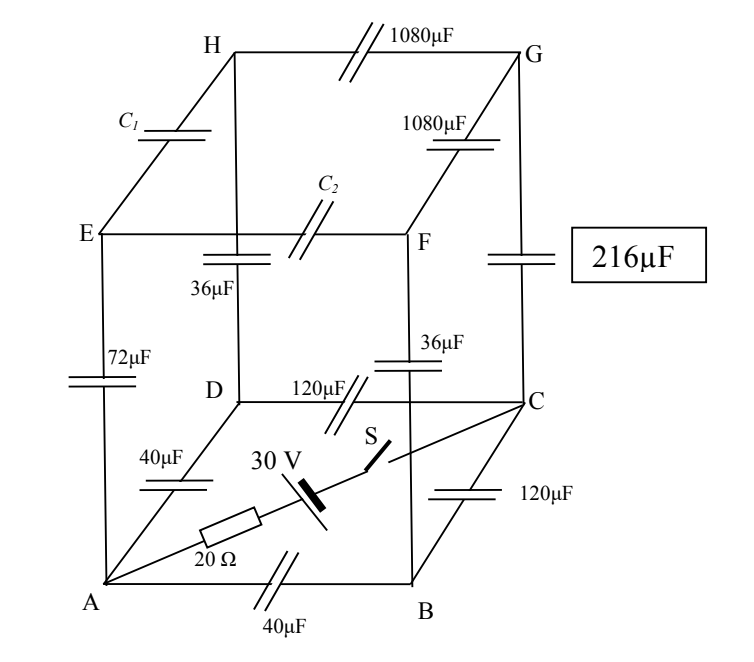
\includegraphics[scale=0.3]{./img/cubo.png}
			\caption{Cubo de Capacitores.}
			\label{ej3}
		\end{figure}
		\textit{Hint: Tome en cuenta que si los capacitores de $36\mu F$ no se cargan es como si no estuvieran, lleve el problema a "2 dimensiones" y busque simetrías.} \\
	\end{ejercicio}
	\textbf{Solución 3: } \\
	Fuck
\end{mdframed}





\begin{mdframed}[style=warning]
	\begin{ejercicio}
		Se construye un acelerómetro eléctrico mediante dos condensadores en serie, de sección cuadrada de lado $L$ y con placas separadas una distancia $a$. Entre los extremos de la asociación se encuentra aplicada una diferencia de potencial constante $V_o$. Un líquido dieléctrico ideal, de permitividad $\varepsilon$, puede pasar de uno a otro condensador. En el estado de movimiento uniforme, el líquido llena hasta la mitad ambos condensadores. Cuando el sistema posee una cierta aceleración, los niveles cambian, de forma que entre los dos condensadores existe un desnivel $h$ relacionado con la aceleración por la ecuación $a/g = h/d$, siendo $d$ la distancia entre los condensadores.
		\begin{enumerate}[a)]
			\item Halle la diferencia de potencial entre las placas del condensador $1$. Calcule la diferencia con su valor para $h = 0$ y, a partir de aquí, obtenga la aceleración del dispositivo.
			\item ¿Cuánto varía la carga del condensador $1$ cuando el desnivel pasa de $0$ a $h$? ¿Y la energía electrostática almacenada en el sistema?
		\end{enumerate}
		\begin{figure}[H]
			\centering
			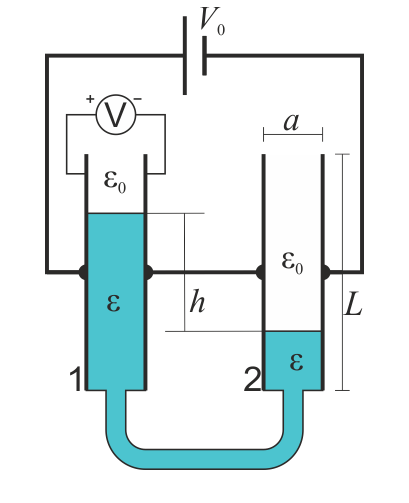
\includegraphics[scale=0.25]{./img/acelerometro.png}
			\caption{Acelerómetro.}
			\label{ej3}
		\end{figure}
	\end{ejercicio}
	\textbf{Solución 4: } \\
	Fuck
\end{mdframed}














































%%%